\chapter{Princip postačitelnosti, podmíněnosti, věrohodnosti, zastavovací pravidlo sekvenčního principu, vztahy.}
\begin{description}
	\item[SUFFICIENCY princip:] Máme $\epsilon$ závislé na~$\t$, pozorování $x,y$ a~nechť je v~$\epsilon$ k~dispozici postačující statistika $T$ (PS). Víme, že $T(x)=T(y)$ a~chceme, aby závěry o~$\t$ na~základě $x$ nebo $y$ byly shodné. ($T$ je PS pokud rozdělení $X|T(X)=t$ nezávisí na~$\t$).

\item[LIKELIHOOD princip:] Informace o~$\t$ nesená $x$ je zcela obsažena ve~všech funkcích ($f_\X(\textbf{x},\t)=L$). Navíc, pokud máme pozorování $x_1$ experimentu $\epsilon_1$ a~$x_2$ v~experimentu $\epsilon_2$ taková, že 
$$ L_1(\t|x_1)=c L_2(\t|x_2),\qquad\forall\t\in\Theta.$$
Chceme, aby závěry o~parametru $\t$ v~obou experimentech byly shodné. označíme $\mathrm{Ev}(\epsilon_1,x_1)=\mathrm{Ev}(\epsilon_2,x_2)$ (Ev jako Evidence). 
\item[CONDITIONALITY princip:] Nechť máme dostupné $\epsilon_1,\epsilon_2$. Definujeme $\epsilon^*$ experiment tak, že vybereme náhodně mezi~$\epsilon_1 \vee \epsilon_2$, a~v~něm měříme $x_1/x_2$. Chceme, aby $\Ev(\epsilon^*,(j,x_j))=\Ev(\epsilon_j,x_j),~\forall j,\forall x_j$.
\item[STOPPING rule:] Máme $\epsilon_1,\epsilon_2$ jako zastavovací pravidlo $\tau$, které zastavuje posloupnost v~$\epsilon_n$. Jsou naměřeny $\textbf{x}=\Big( x_1^{\epsilon_1},x_2^{\epsilon_2},...,x_n^{\epsilon_n} \Big)$, ozn. $\{ \epsilon_1,...,\epsilon_n,\tau \}$ (sekvenční). Chceme, aby $\Ev\Big( \{ \epsilon_1,...,\epsilon_n,\tau \},\textbf{x} \Big)$ zvisela na~$\tau$ pouze prostřednictvím $\textbf{x}$, tzn. $$\Ev\Big( \{ \epsilon_1,...,\epsilon_n,\tau_1 \},\textbf{x} \Big)=\Ev\Big( \{ \epsilon_1,...,\epsilon_n,\tau_2 \},\textbf{x} \Big),~\forall \textbf{x}.$$
\item[BAYESOVSKÝ princip:] Taková procedůra, která využívá k~rozhodnutí o~parametru $\t$ aposteriorní hustotu $\pi(\t,\textbf{x})=\frac{f_\X\cdot\pi(\t)}{\int f_\X\cdot\pi(\t) d\t}$, např. $\widehat{\t}_B=''\EE{\pi(\t,\textbf{x})}''=\E^\pi(\t)$.
\end{description}

\begin{example}[STOPPING rule]
	Mějme $\epsilon_j..x_j\in\Ran(X_j)$, kde $X_j\sim f(x_j,\t),~\forall j\in 1,2,...$. Teoricky můžeme jít až do~nekonečna, ale někdy chceme experiment zastavit, abychom mohli vyhodnotit data. Definujeme tedy $\tau$ jako zastavení v~bodě $n$, pokud $\textbf{x}:=(x_1,...,x_n)\in\Ran(X_1)\times\Ran(X_2)\times...\times\Ran(X_n)\equal{ozn}\Aa_n$. Platí, že
	$$ L(\t|\textbf{x})\equal{id}\Big(\prod f_{X_j}(x_j,\t) \Big)\cdot I_{\Aa_n}(\textbf{x})=f(x_1|\t)f(x_2|x_1,\t)...f(x_n|x_1,x_2,...,x_{n-1},\t)I_{\Aa_n}(\textbf{x}).$$
	$\tau_1,\tau_2... \textbf{x}(\epsilon_n)$ (!! prosím o~intro). Pokud platí $L$, potom platí $SR$, tedy ($L_1^{(\tau_1)}=L_2^{(\tau_2)}$).
\end{example}
\begin{example}[BAYESOVSKÝ princip]
	Máme TV seriál. Označme $\t\in[0,1]$ jako podíl diváků, kteří daný seriál sledují. Bylo zjištěno, že 9 diváků seriál sledují a~3 nikoliv (to jsou naše data). Problém je, že nevíme, jakým způsobem byla data naměřena. 
	\begin{description}
		\item[$\epsilon_\mathrm{I}:$] vybráno $n=12$ lidí - test (9DIV,3NEDIV). Máme tedy náhodnou veličinu $X$ jako počet diváků z~$n=12$ nezávislých opakování. Z~toho plyne, že $X\sim \Bi(12,\t)$. Máme napozorováno $X(\omega)=x=9$.
		\item[$\epsilon_\mathrm{II}:$] vybíráme $N$ osob a~testujeme, dokud nezískáme $3$ nediváky. Při~tomto způsobu ale měření probíhá zcela odlišně. Tedy $N\sim\mathrm{NegBi}(3,1-\t)$. Napozorováno tedy bylo $N(\omega)=n=12$.
	\end{description}
$$ L_\mathrm{I}(\t,\epsilon_\mathrm{I})=c_1\t^9(1-\t)^3\quad\propto\quad L_\mathrm{II}(\t,\epsilon_\mathrm{II})=c_2\t^9(1-\t)^3,\quad \forall\t\in[0,1] $$
Z toho pro~LIKELIHOOD vyplývá, že $\Ev(\epsilon_\mathrm{I},(9/??))=\Ev(\epsilon_\mathrm{II},(12))$ (takže vlastně na~zastavovacím principu nezáleželo).
\end{example}

\begin{example}
	Máme laboratoř a~v~ní dva přístroje. Jako $\t$ označme\begin{itemize}
		\item 1. přístroj přesný $X_1\sim\NN(\t,0.1)$ [$\epsilon_1$] (vytížený)
		\item 2. přístroj nepřesný $X_2\sim\NN(\t,10)$ [$\epsilon_2$] (volný)
	\end{itemize}
Rozhodování o~$\t$: 95\%-interval spolehlivosti pro~$\t$\begin{enumerate}[A)]
	\item osobně. naměříme $x_1$ jako délka($IS_{95\%}$)$=0.62$ (na 2.př. nezáviselo).
	\item vyšleme laborantku. která nese data (ale neví, ze~kterého přístroje jsou, prostě použila volný přístroj). $\beta\in(0,1)$. Máme model $\Phi=\beta\NN(\t,0.1)+(1-\beta)\NN(\t,10).$ Pak zjistíme $x$ jako délku($IS_{95\%}$) s~hodnotou $5.19$.
\end{enumerate}
\end{example}
\begin{theorem}
	$S\wedge C\Leftrightarrow L\Rightarrow SR$. Implikace $S\Rightarrow C$ je důležitá, protože $B''\Rightarrow'' L$.
	\begin{proof}
		Mějme $\epsilon_1,\epsilon_2$, $x_1,x_2$ a~předpokládejme, že $L_1(\t)=c L_2(\t)$. Ptáme se, jestli je $\Ev(\epsilon_1,x_1)=\Ev(\epsilon_2,x_2)$. Víme, že $$ \underbrace{\pi_1(\t,x_1)}_{\epsilon_1}=\frac{f_X(x_1,\t)\pi(\t)}{\int f_X(x_1,\t)\pi(\t)\d\t}=\frac{c f_{X_2}\pi}{\int c f_{X_2}\pi\d\t}=\underbrace{\pi_2(\t| x_2)}_{\epsilon_2}.$$
	\end{proof}
\begin{proof}[$L\Rightarrow S$]
	Nechť T je PS($\epsilon$) a~nechť máme data $x_1^0,x_2^0$ (nula značí konkrétní výběr, nikoliv obecný), taková, že $T(x_1^0)=T(x_2^0)$. Máme k~dispozici Neymannův faktorizační teorém, $X\sim f(x,\t)$, pak $T(X)$ je PS právě tehdy, když $f(x|\t)=h(x)g\big(T(x),\t \big),~\forall\t$. Potom tedy 
	$$ L(\t|x_1^0)=f(x_1^0,\t)=h(x_1^0)g\big( T(x_1^0),\t \big)=\frac{h(x_1^0)}{h(x_2^0)}\underbrace{h(x_2^0)g\big(T(x_2^0),\t \big)}_{f(x_2^0,\t)=L(\t,x_2^0)},\quad\forall\t.$$
	Z toho vyplývá, že dle principu L platí, že $\Ev(\epsilon,x_1^0)=\Ev(\epsilon,x_2^0)$.
	
	
	!!!všude velké l pokud není, TODO!!
\end{proof}
\begin{proof}[$L\Rightarrow C$]
Uvažujeme experiment $\epsilon^*$ tak, že $(\mathrm{I},X_\mathrm{I})=X^*$, $(\forall j\in\{1,2\},~\forall x_1,x_2)$, tedy $$\Ev\big(\epsilon^*,(j,x_j) \big)=\Ev\big(\epsilon_j,x_j \big).$$
Dále potom $$ L^*(\t|\underbrace{j,x_j}_{X^*})=\PP\big(X^*=(j,x_j) \big)=\PP(I=j\wedge X_{I=j}=x_j)=\PP(I=j)\PP(X_j=x_j)=0.5f(x_j,\t)=0.5 L_j(\t,x_j).$$
Potom 
$$L^*=c L_j,~ \forall j,\forall x_j\quad\Rightarrow\quad\Ev\big(\epsilon^*,(j,x_j) \big)=\Ev\big(\epsilon_j,x_j \big).$$
\end{proof}
\end{theorem}

Statistical decision theory:

\begin{define}
	Označíme $\Dd$ jako množinu možných rozhodnutí o~$\t$, případně $\tau(\t)$. Dále potom $\delta\in\Dd$. $L:\Theta\times\Dd\to[0,+\infty)$ nazýváme \textbf{loss function} (ztrátová funkce) a~$L(\t,\delta)$ jako \textbf{míru ztráty} (shody, neshody), pokud pro~$\t$ použijeme rozhodnutí $\delta$.
	
	Označme dále $\Rr$ jako \textbf{reward space}, který je spojen s~$\Dd$,tj. $\forall\delta\in\Dd$ přiřazuje $r\in\Rr$ ($\delta\leftrightarrow r$). Předpokládejme dále, že na~$\Rr$ existuje úplné uspořádání ($\leq$) tak, že \begin{enumerate}[A1)]
		\item $\forall r_1,r_2\in\Rr,~r_1\leq r_2 \vee r_2\leq r_1$,
		\item $\forall r_1,r_2,r_3\in\Rr,~r_1\leq r_2 \wedge r_2\leq r_3~\Rightarrow~r_1\leq r_3$. Z~toho vyplývá, že 
		$$ r_1<r_2,\quad r_2<r_1,\quad r_1=r_2~(r_1\sim r_2).$$
		Poslední rovnost není myšlena jako číselná rovnost, ale spíše jako ekvivalence (peníze pro~nás můžou mít stejnou cenu, jako získané znalosti).
	\end{enumerate}
Nad $\Rr$ definujeme prostor $\mathcal{P}$ jako pravděpodobnostní distribuci $\{\PP\}$ nad~$r$ ($r\sim\PP\in\mathcal{P}$). Předpokládejme, že na~$\mathcal{P}$ existuje úplné uspořádání ($\leq$) takové, že ...
\end{define}

Motivace: označme $d_i$ jako investice do~$i$-té společnosti. Na~konci roku pak očekáváme dividenda $r_i$. $(d_i)_1^k...(r_i)_1^k...r_i\sim \PP_1\ast\PP_k$ (CLT)..

\section{15.10.}
\begin{define}
	Funkci $U$ na~$\R$ nazveme \textbf{užitkovou} (utility function), pokud $\forall P,Q\in\mathcal{P}$ platí, že 
	$$ P\leq Q\quad\Leftrightarrow\quad\E^P\big[U(r)\big]\leq\E^Q\big[U(r)\big],$$ kde $r$ je náhodná veličina, pro~kterou $U(r)=r$.
\end{define}
\begin{remark}
	Pokud má $\mathcal{P}$ vhodné vlastnosti, pak existuje užitková funkce $U(r)$, která zachovává dané uspořádání $\mathcal{P}$. 
\end{remark}
\begin{remark}
	\begin{enumerate}[a)]
		\item Pro~ztrátu $L(\t,\delta)$ platí, že $L(\t,\delta)=U(\t,\delta)=-\E[U(r)]+c$, kde konstantu $c$ přičítáme proto, abychom se~nedostali do~záporných čísel. Tím zajistíme??? minimalizaci $L\sim\max$ užitku.
		\item Předpověď počasí v~Kanadě. Předpovědi jsou ve~tvaru "pravděpodobnost, že zítra bude pršet je $p$". Předpovědi od~$N$ různých společností chceme nějak porovnat. Sledujeme tedy 365 dní všechny předpovědi a~přiřadíme jim $p_1,...,p_N$. Definujeme relativní četnost $$\t_j=\frac{\text{\# dnů, kdy pršelo a~byla použita }p_j}{\text{\# dnů, kdy byla použita }p_j},j\in\widehat{N}.$$ Sestavíme ztrátovou funkci (poprvé použil De Grout v~roce 1988) $$L(\t,p)=\sumjn q_j(\underbrace{p_j-\t_j}_{H(q)})^2+\sum_{i=1}^N q_i\ln q_i,$$ kde $q_j=\frac{\text{\# použití }p_j}{365}$ a~$H(q)=-\sum_1^J q_j\ln q_j\geq 0$, kde ${q_j}_1^J$ jsou rozdělení pravděpodobnosti. Suma $\sum_{i=1}^N q_i\ln q_i$ pak penalizuje předpovědi, které jsou nevyvážené.
		
		Pokud bychom měli systém neuspořádanosti, pak by bylo $H(\textbf{q})$ maximální. O~$\textbf{q}$ víme, e má rovnoměrné rozdělení $q_j=\frac{1}{J}$.
	\end{enumerate}
\end{remark}
\begin{remark}
	Člen $\sumjn q_j(p_j-\t_j)^2$ v~minulé poznámce nemusí nutně být na~druhou, můžeme brát závorku i~v~absolutní hodnotě, případně ji umocnit na~$\alpha$. Zde vstupuju do~našeho problému tzv. \textbf{Apriorno}. Musíme totiž dopředu vědět některé informace, třeba $X\sim f(x,\t),~L(\t,\delta)$.
\end{remark}
\begin{define}
	Mějme $\Theta$, $\mathcal{F}=\big\{ f(x,\t):\t\in\Theta \big\}$,~$\mathscr{D}$, kde $\delta\in\mathscr{D}$ a~$\chi$ jako výběrový prostor s~daty $\textbf{x}$.
	
	Funkci $\delta:\chi\to\mathscr{D}$ nazýváme \textbf{rozhodovací funkce}, $\delta(\textbf{x})=\delta\in\mathscr{D}$. 
\end{define}
\begin{description}
	\item[Metoda A) minimalizace L] Máme $\delta_L(\textbf{x})=\argmin\limits_{\delta\in\mathscr{D}} L\big(\t,\delta(\textbf{x})\big),~\forall \t\in\Theta,~\forall\textbf{x}\in\chi$. (vynechal jsem prezentace)
	\item[Metoda B) Riziková funkce] (risk function) je funkce $\mathcal{R}:\Theta\to\R^+$ definovaná jako $$\mathcal{R}(\t,\delta)=\E_\t L\big(\t,\delta(\textbf{X})\big)=\int L\big(\t,\delta(\textbf{x})\big)f_\textbf{X}(\textbf{x},\t)\d\textbf{x}.$$
	Rizikovou funkci také nazýváme jako \textit{střední ztrátu}. Dále definujeme $\delta_U=\argmin\limits_{\delta\in\mathscr{D}} \mathcal{R}(\t,\delta),~\forall\t\in\Theta$.
\begin{figure}[h]
	\centering
	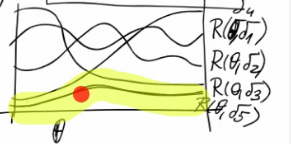
\includegraphics[width=0.5\linewidth]{pictures/P4_1}
	\caption{chybí popis}
	\label{fig:p41}
\end{figure}\begin{figure}[h]
\centering
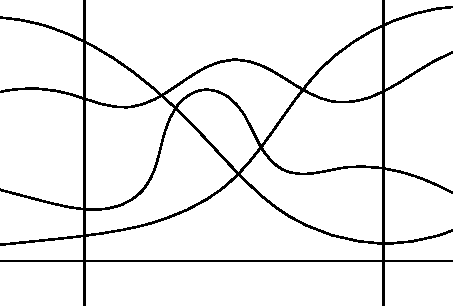
\includegraphics[width=7cm,height=3cm]{pictures/P4_1v2}
\caption{template pro Filipa ;)}
\label{fig:p41v2}
\end{figure}
Řešením je potom $\mathscr{D}_0\subset\mathscr{D}$ minimální na~??? $\mathscr{D}_0$.\begin{enumerate}[a)]
	\item  Prostor rozhodovacích funkcí, které jsou nestranné pak vede na~UMVUE.
	\item $\mathscr{D}_0$ je invariantní rozhodovací funkcí na~určitou transformaci (lokálně-měřítkové modely) (nemám páru co jsem to psal :D díky~za~opravu)
\end{enumerate}

Problémy: \begin{enumerate}[a)]
	\item $\delta_1,\delta_2$, $\mathcal{R}(\t,\delta_1$ a~$\mathcal{R}(\t,\delta_2)$) .. tady mi to chybí
\end{enumerate}
\end{description}

\begin{example}
	Mějme $X=\begin{cases}
	\t-1,& \PP=\frac{1}{2}, \\ \t+1,& \PP=\frac{1}{2},
	\end{cases}~\t\in\R,~\mathscr{D}=\R$. Potom
	$ L(\t,\delta)=1-I_\t(\delta)$ nazýváme "0-1" ztrátovou funkci, viz obrázek \ref{fig:p42}.
	\begin{figure}[h]
		\centering
		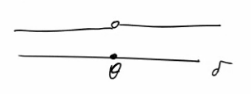
\includegraphics[width=0.4\linewidth]{pictures/P4_2}
		\caption{nic}
		\label{fig:p42}
	\end{figure}
	\begin{enumerate}[1)]
		\item Máme $(x_1,x_2)$ data a~sestrojíme $\delta_0=\frac{x_1+x_2}{2}=\begin{cases}
		\t\\\t-1\\\t+1
		\end{cases}$ symetricky kolem~$\t$. Potom
		$$ \mathcal{R}(\t,\delta_0)=\E L(\t,\delta_0)=1-\E I_\t(\delta_0)=1-\PP(\delta_0=\t)=1-\PP(X_1\neq X_2)=\frac{1}{2}.$$ To nám říká, že střední ztráta je rovna $\frac{1}{2}$. V~průměru tedy 50\% případu bude příznivá (trefíme se~do~parametru).
		\item Máme data $(x_1,x_2)$ a~sestrojíme $\delta_1=x_1+1=\begin{cases}
		\t\\\t+2
		\end{cases}$ nesymetricky rozdělené kolem~$\t$. Potom
		$$\mathcal{R}(\t,\delta_1)=...=1-\PP(\delta_1=\t).$$
	\end{enumerate}
Srovnání $\delta_0$ a~$\delta_1$ nelze rozhodnout na~základě $\mathcal{R}$-strategie. Můžeme na~ně však využít např. UMVUE, MREE nebo N-P lemma.
\end{example}
\begin{description}
	\item[Metoda c) Strategie MINIMAXní] $\sup\limits_{\t\in\Theta} \mathcal{R}(\t,\delta)$ nazýváme \textit{maxní} riziková funkce a~je rovna $\mathcal{R}_{\sup}(\t,\delta)$. Definujeme 
	$$ \delta_0=\argmin\limits_{\delta\in\mathscr{D}}\mathcal{R}_{\sup}(\t,\delta)=\argmin\limits_{\delta\in\mathscr{D}}\underbrace{\sup\limits_{\t\in\Theta}\underbrace{\E_\t L(\t,\delta(\X))}_{\mathcal{R}(\t,\delta)}}_{r_{\sup}\in\R_0^+}.$$
\end{description}

\begin{define}
	Definujeme \textbf{minimaxní riziko} ve~tvaru $\overline{\mathcal{R}}=\inf\limits_\delta\sup\limits_\t\mathcal{R}(\t,\delta)$.
\end{define}
\newpage
\begin{figure}[h]
	\centering
	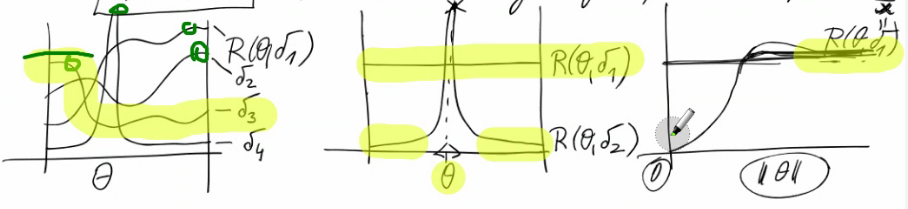
\includegraphics[width=0.95\linewidth]{pictures/P4_3}
	\caption{1: zeleně suprema, nejmenší supremum je delta3 2: lepší je delta2, protože ač je riziko vysoké, jeho šance je velice malá - toto je nevýhoda minimaxní strategie 3: delta2 jen lehce překmitne delta1 a pak se k němu blíží asymptoticky}
	\label{fig:p43}
\end{figure}



\begin{remark}
	Analogie z~teorie her. Pokud máme 2 hráče, kteří mají antagonický vztah (snaží se~navzájem poškodit a~nezáleží jim na~ztrátě). První hráč udělá nějaký tah. Druhý hráč pak udělá tah, který co nejvíc poškodí 1. hráče. První hráč to předvídá a~snaží se~tedy minimalizovat nejhorší možnou ztrátu.
\end{remark}

